% ICML 2026 AI for Math Workshop poster.
% Size: 24 in (W) x 36 in (H) portrait = 61 cm x 91 cm.
% Compile with: tectonic poster.tex   (or pdflatex/xelatex)

\documentclass[final]{beamer}

\usepackage[orientation=portrait,size=custom,width=61,height=91,scale=1.05]{beamerposter}
\usepackage[utf8]{inputenc}
\usepackage[T1]{fontenc}
\usepackage{lmodern}
\usepackage{microtype}
\usepackage{booktabs}
\usepackage{graphicx}
\usepackage{xcolor}
\usepackage{tikz}
\usepackage{qrcode}
\usepackage{ragged2e}
\usepackage{array}

% --- Palette (matches docs/index.html: monochrome) ---------------------
\definecolor{fg}{HTML}{111111}
\definecolor{muted}{HTML}{6e6e6e}
\definecolor{rule}{HTML}{c8c8c8}
\definecolor{accent}{HTML}{4C72B0}   % matches figures (B-RL blue)
\definecolor{warn}{HTML}{DD8452}     % matches figures (A-RL orange)

% --- Beamer theme overrides --------------------------------------------
\setbeamercolor{block title}{fg=fg,bg=white}
\setbeamercolor{block body}{fg=fg,bg=white}
\setbeamerfont{block title}{size=\Large,series=\bfseries}
\setbeamerfont{block body}{size=\normalsize}
\setbeamertemplate{itemize items}{\raisebox{0.25ex}{\tiny$\blacksquare$}}
\setbeamertemplate{navigation symbols}{}
\setbeamertemplate{caption}[numbered]

% --- Layout helpers ----------------------------------------------------
\newcommand{\hr}{\par\noindent\textcolor{rule}{\rule{\linewidth}{0.5pt}}\par}
\newcommand{\bignum}[1]{\textcolor{accent}{\textbf{#1}}}

\title{Inference-Time Diversity in RL-Trained Lean Theorem Provers}
\subtitle{A Diagnostic Study}
\author{Zachary Burton}
\institute{MIT \textquotesingle 26 \quad \texttt{zacburton@alum.mit.edu}}

\begin{document}
\begin{frame}[t]{}

% ============================================================
% HEADER
% ============================================================
\begin{minipage}[c]{0.72\linewidth}
  \raggedright
  {\fontsize{50}{56}\selectfont\bfseries Inference-Time Diversity in\\RL-Trained Lean Theorem Provers}\\[0.3em]
  {\fontsize{28}{34}\selectfont\itshape\color{muted} A Diagnostic Study}\\[0.4em]
  {\Large\bfseries Zachary Burton} \quad
  {\large MIT \textquotesingle 26} \quad
  {\large\texttt{zacburton@alum.mit.edu}}\\[0.15em]
  {\large\color{muted} ICML 2026 \textbullet{} AI for Math Workshop \textbullet{} July 11, COEX Hall D1, Seoul}
\end{minipage}\hfill
\begin{minipage}[c]{0.22\linewidth}
  \raggedleft
  \begin{tikzpicture}
    \node[draw=rule,line width=0.6pt,inner sep=0.2cm] {
      \begin{minipage}{6.5cm}\centering
        \qrcode[height=5.2cm]{https://arxiv.org/abs/2601.16172}\\[0.2em]
        {\footnotesize\color{muted}arXiv:2601.16172}
      \end{minipage}
    };
  \end{tikzpicture}
\end{minipage}

\vspace{0.4cm}
\hr
\vspace{0.4cm}

% ============================================================
% TL;DR
% ============================================================
\begin{tikzpicture}
  \node[draw=fg,line width=1pt,inner sep=0.5cm,fill=white]
    {\begin{minipage}{0.95\linewidth}\centering
      {\Large\bfseries TL;DR\quad}
      {\Large\itshape RL-trained Lean theorem provers run out of ideas as you sample more. A fixed schedule of 15 tactic skeletons closes the gap, and the effect is RL-specific.}
    \end{minipage}};
\end{tikzpicture}

\vspace{0.5cm}

% ============================================================
% 2-COLUMN BODY
% ============================================================
\begin{columns}[t,totalwidth=\linewidth]

% ---------- LEFT COLUMN ----------
\begin{column}{0.485\linewidth}

\begin{block}{Setup}
\justifying
\textbf{Model:} DeepSeek-Prover-V1.5-RL (7B, paired with non-RL V1.5-Base).\\
\textbf{Benchmark:} miniF2F-test (244 Lean 4 / Mathlib theorems).\\
\textbf{Schedule:} 15 hand-picked tactic skeletons (\texttt{simp}, \texttt{intro},
\texttt{constructor}, \texttt{aesop}, \dots) $\times$ 8 NL goal hints
= 120-slot grid. Budgets $k \in \{16,32,64\}$ take the first $k$ slots.\\
\textbf{Decoding:} temperature 0.6, top-$p$ 0.95, max 1024 tokens.
\textbf{Verifier:} \texttt{lake env lean --json}, 120\,s timeout,
8-way sharding by $i \bmod 8$.
\end{block}

\begin{block}{Mode collapse: A-RL plateaus at $k{=}32$}
\begin{center}
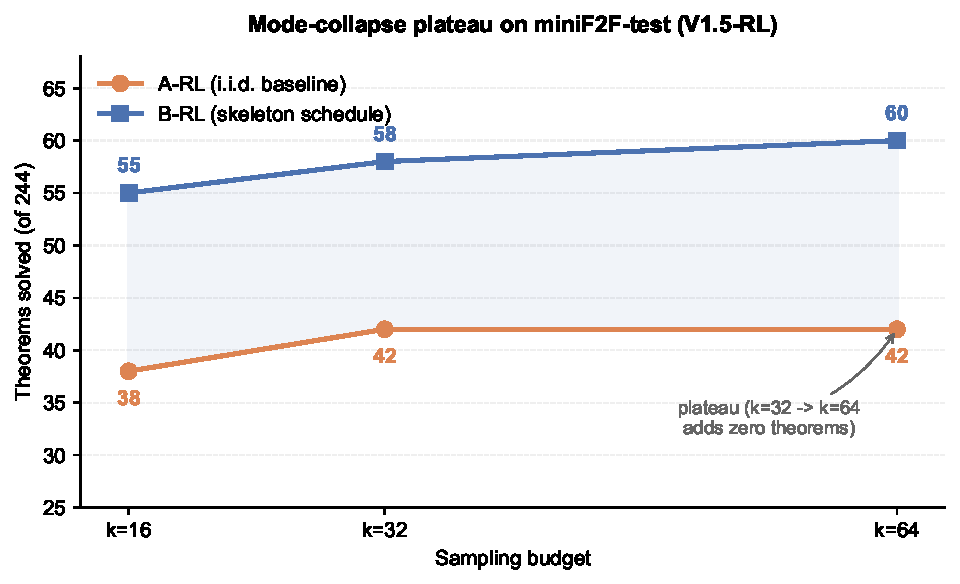
\includegraphics[width=\linewidth]{../figures/scaling.pdf}
\end{center}

\vspace{0.3em}
\centering
\renewcommand{\arraystretch}{1.15}
\begin{tabular}{lccc}
\toprule
                              & $k{=}16$       & $k{=}32$       & $k{=}64$       \\ \midrule
A-RL (i.i.d.)                 & 38/244 (15.6\%) & 42/244 (17.2\%) & 42/244 (17.2\%) \\
\textbf{B-RL (skeleton)}      & \textbf{55} (22.5\%) & \textbf{58} (23.8\%) & \textbf{60} (24.6\%) \\
$\Delta$ absolute             & $+17$           & $+16$           & $+18$           \\
$\Delta$ relative             & $+44.7\%$       & $+38.1\%$       & $+42.9\%$       \\
\bottomrule
\end{tabular}\\[0.4em]
\justifying\small\color{muted}
Across-seed: mean $\Delta = +12.3 \pm 4.2$ theorems at $k{=}16$ ($n{=}3$ seeds, sign positive every seed).
\end{block}

\begin{block}{Diversity ablation: structural content drives the gain}
\begin{center}
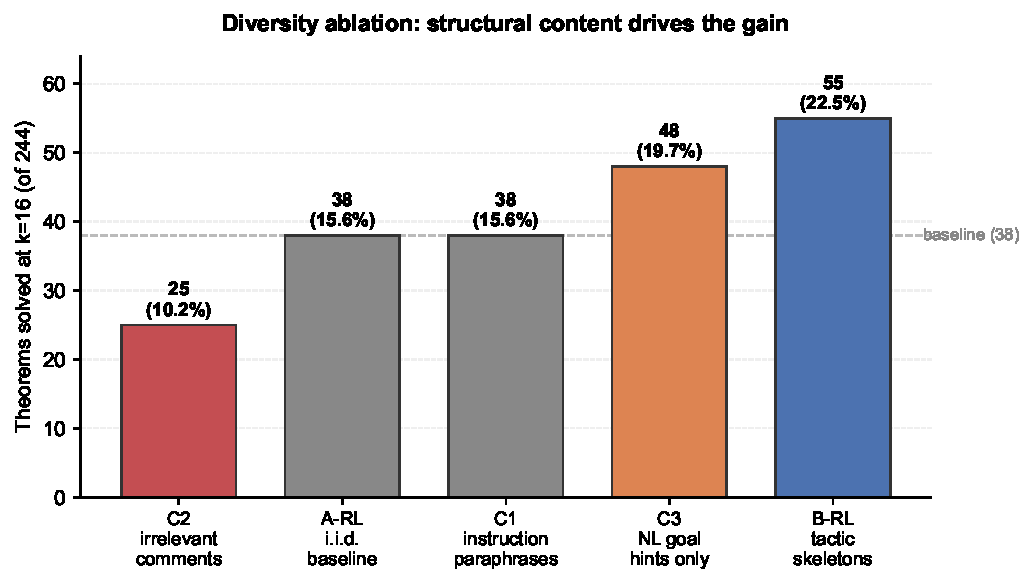
\includegraphics[width=\linewidth]{../figures/ablation.pdf}
\end{center}
\justifying\small
\textbf{C2 < A-RL = C1 < C3 < B-RL.} Irrelevant Lean comments \emph{hurt};
paraphrased instructions match the baseline; NL goal hints recover 58\% of the
A$\to$B gap; tactic skeletons go furthest. The gain is structural, not just
diversity.
\end{block}

\end{column}

% ---------- RIGHT COLUMN ----------
\begin{column}{0.485\linewidth}

\begin{block}{Solved-set overlap (V1.5-RL, $k{=}16$)}
\begin{center}
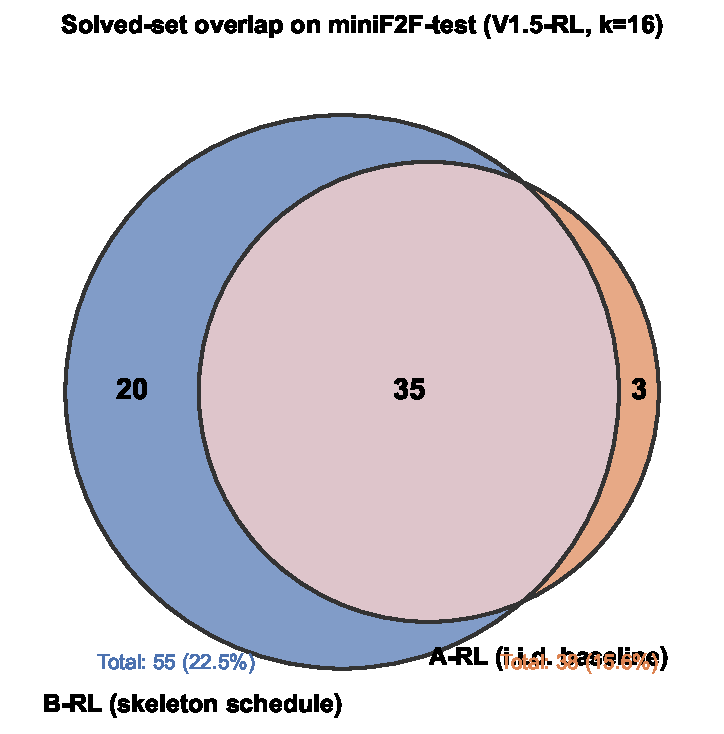
\includegraphics[width=0.72\linewidth]{../figures/venn_overlap.pdf}
\end{center}
\justifying\small
B-RL nearly Pareto-dominates A-RL: \bignum{20} theorems are solved only by B-RL,
\bignum{3} only by A-RL, \bignum{35} by both.
\end{block}

\begin{block}{Phenomenon is RL-specific}
\justifying
DeepSeek-Prover-V1.5-Base (the same model, no RL fine-tune) proves
\textbf{0/244} theorems at every $k$, with \emph{or} without skeletons.
\begin{itemize}
\item Base outputs \texttt{sorry} or echoes the statement in 58.8\% of attempts.
\item RL model emits \texttt{sorry} in $<\!0.2\%$ of attempts; its mode collapse
  manifests as persistent generation of failing-but-valid \texttt{rw}/\texttt{apply}
  sequences.
\end{itemize}
\textbf{RL is the locus of both the proof capability and the inference-time
collapse that limits it.}
\end{block}

\begin{block}{Per-skeleton contribution (within $k{=}16$)}
\begin{center}
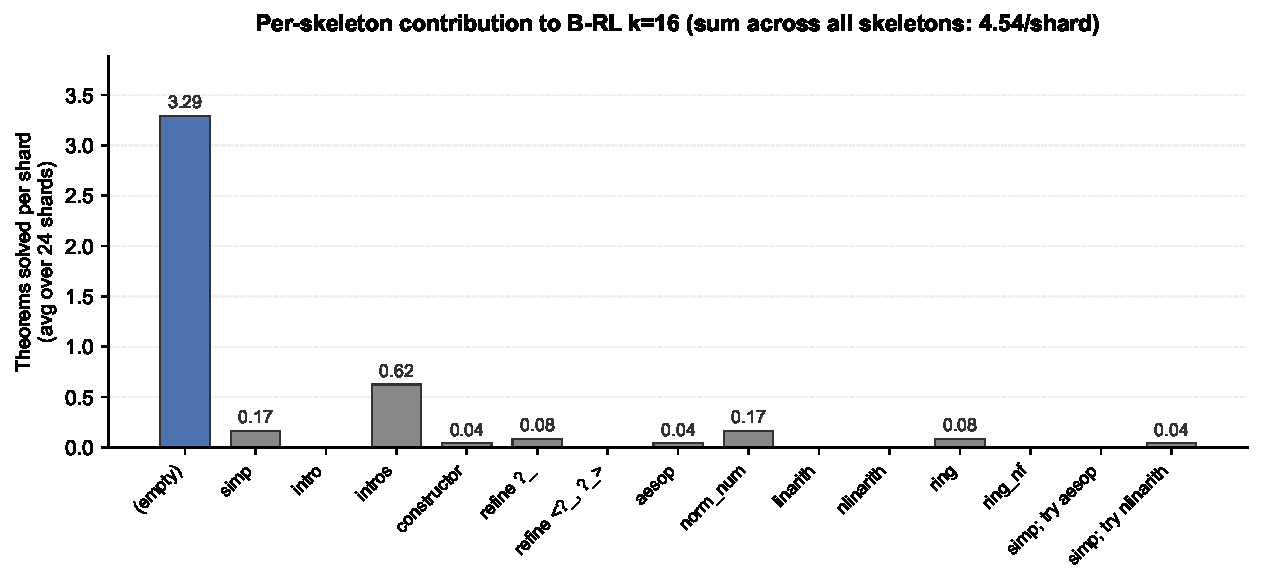
\includegraphics[width=\linewidth]{../figures/per_skeleton.pdf}
\end{center}
\justifying\small
24 B-RL $k{=}16$ shards, within-shard counting. Empty skeleton carries most of the load
(3.29/4.54 solves per shard); the other 14 skeletons together pick up the long
tail $-$ exactly the 17 theorems A-RL i.i.d.\ misses.
\end{block}

\begin{block}{Cross-model generalisation}
\justifying
A$\to$B contrast on two further 7B Lean provers:
\begin{itemize}
\item \textbf{RL-trained V2-7B:} $+3$ \emph{frontier} theorems no i.i.d.\
  baseline of any tested model reaches.
\item \textbf{SFT Goedel-Prover:} $\mathbf{-10.0 \pm 4.4}$ theorems
  ($n{=}3$ seeds, negative every seed). The intervention helps RL and
  \emph{hurts} SFT.
\end{itemize}
\end{block}

\end{column}
\end{columns}

\vspace{0.3cm}

% ============================================================
% DISTRIBUTIONAL STRIP (full-width, below the 2 columns)
% ============================================================
\begin{tikzpicture}
  \node[draw=fg,line width=0.6pt,inner sep=0.4cm,fill=white]
    {\begin{minipage}{0.95\linewidth}\centering
      {\Large\bfseries Distributional evidence of collapse:\quad}
      {\Large Across \bignum{13{,}159} stochastic V1.5-RL samples, the median theorem gets only \bignum{2} distinct first-tactic heads; \bignum{49\%} of the benchmark gets a deterministic single strategic opening.}
    \end{minipage}};
\end{tikzpicture}

% ============================================================
% FOOTER
% ============================================================
\vfill
\hr
\vspace{0.3cm}
\begin{minipage}[c]{0.88\linewidth}
  \raggedright
  \large
  \textbf{Code, prompts, per-attempt logs:}
  \texttt{github.com/zacn04/icml\_hints\_for\_provers}\\[0.1em]
  \textcolor{muted}{Lean 4 v4.9.0-rc1 \textbullet{} Mathlib pinned \textbullet{}
  outputs/ run dirs are deterministic SHA-prefixes of the experiment config}
\end{minipage}\hfill
\begin{minipage}[c]{0.10\linewidth}
  \raggedleft
  \qrcode[height=2.2cm]{https://github.com/zacn04/icml_hints_for_provers}
\end{minipage}

\end{frame}
\end{document}
